\section{The Generated Datasets}\label{sec:description}

%  |- [0] p10(X0,X1) :- p3(X1,X2),p5(X0,X1).
% 	|- [1] p5(X0,X1) :- p7(X1,X0).
% 		|- [2] p7(X1,X0) :- p2(X3,X1),p2(X4,X0).

\begin{figure*}[t!]
    \centering
    \subfigure[Chain]{%Chain (dataset CHAIN-S-3)
        \centering
        \fbox{
        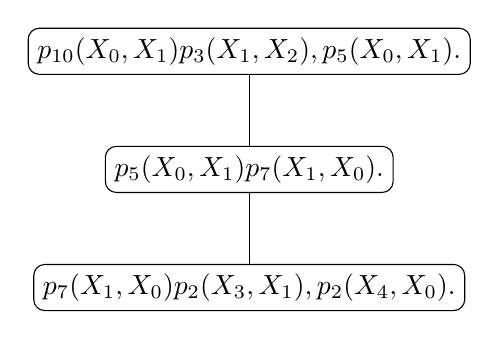
\begin{tikzpicture}[sibling distance=10em,every node/.style = {shape=rectangle, rounded corners, draw, align=center, top color=white}]]%, bottom color=blue!20
            \node {$p_{10}(X_0,X_1) \ass {p_3(X_1,X_2)},p_{5}(X_0,X_1).$}
            child { node {$%\mathbf
            {p_{5}(X_0,X_1)}\ass {p_{7}(X_1,X_0)}.$} edge from parent%[->]
            child { node {$%\mathbf
            {p_{7}(X_1,X_0)} \ass p_2(X_3,X_1),p_{2}(X_4,X_0).$} edge from parent%[->]
            } };
        \end{tikzpicture}}
       }
%   
%  |- [0] p6(X0,X1) :- p3(X2,X1),p2(X0,X2).
% 	|- [1] p3(X2,X1) :- p4(X2,X1).
% 		|- [3] p4(X2,X1) :- p10(X2,X1).
% 	|- [2] p2(X0,X2) :- p7(X2,X0).
% 		|- [4] p7(X2,X0) :- p8(X2,X0).
  \subfigure[Rooted DG]{
        \centering
        \fbox{
        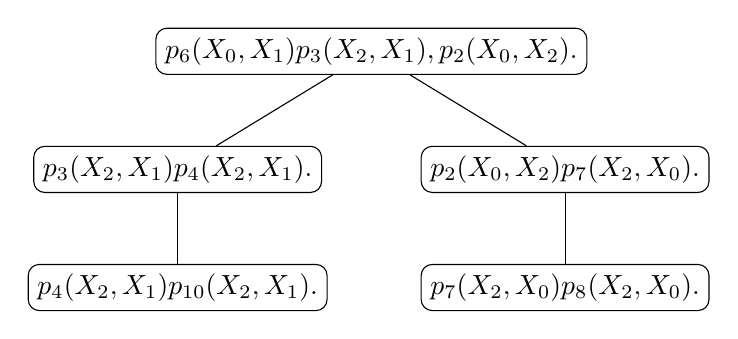
\begin{tikzpicture}[sibling distance=14em,
        every node/.style = {shape=rectangle, rounded corners,
        draw, align=center,
        top color=white}]]%, bottom color=blue!20
            \node {$p_6(X_0,X_1) \ass p_3(X_2,X_1),p_2(X_0,X_2).$}
            child { node {$p_3(X_2,X_1) \ass p_4(X_2,X_1).$} 
            child { node {$p_{4}(X_2,X_1) \ass p_{10}(X_2,X_1).$}}}
            child { node {$p_2(X_0,X_2) \ass p_7(X_2,X_0).$}
            child { node {$p_{7}(X_2,X_0) \ass p_{8}(X_2,X_0).$}}};
        \end{tikzpicture}}
    }
    % 
%      |- [0] p2(X0,X1) :- p6(X0,X1).
% 	|- [1] p6(X0,X1) :- p4(X2,X0),p8(X0,X1).
% 		|- [2] OR
% 			|- [3] p4(X2,X0) :- p4(X0,X3),p3(X2).
% 			|- [4] p4(X2,X0) :- p3(X0),p9(X2,X0).
    \subfigure[Disjunctive Rooted DG]{
        \centering
        \fbox{
        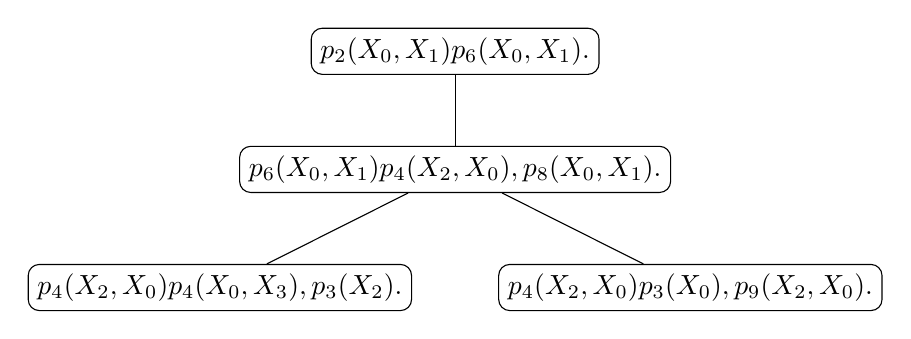
\begin{tikzpicture}[sibling distance=17em,
        every node/.style = {shape=rectangle, rounded corners,
        draw, align=center,
        top color=white}]]%, bottom color=blue!20
            \node {$p_2(X_0,X_1) \ass p_6(X_0,X_1).$}
            child { node {$p_6(X_0,X_1) \ass p_4(X_2,X_0),p_8(X_0,X_1).$} 
           % child[node distance=0.01mm] { node[node distance=0.01mm]{}
            % %
            child { node {$p_4(X_2,X_0) \ass p_4(X_0,X_3),p_3(X_2).$} }
             child { node {$p_4(X_2,X_0) \ass p_3(X_0),p_9(X_2,X_0).$}}        %}
             };
        \end{tikzpicture}}
    }
    \caption{Example rule sets generated for the different categories (the rules of datasets
    (a) CHAIN-S, (b) RDG-S, (c) DRDG-XS).}
    % Categories (a) Chain, (b) Rooted DG, and (c) Disjunctive Rooted DG}
    \label{fig:datasets}
\end{figure*}



% \begin{figure}
% \centering
% % |- [0] p0(X0,X1) :- p3(X1),p18(X0).
% %  |- [1] p18(X0) :- p15(X0,c46).
% %   |- [2] p15(X0,X2) :- p4(X2),p11(X0).
% \fbox{
% \begin{tikzpicture}[sibling distance=10em,
% every node/.style = {shape=rectangle, rounded corners,
% draw, align=center,
% top color=white}]]%, bottom color=blue!20
% \node {$p_0(X_0,X_1) \ass p_3(X_1),p_{18}(X_0)$}
% child { node {$p_{18}(X_0) \ass p_{15}(X_0,c_{46})$} edge from parent[->]
% child { node {$p_{15}(X_0,X_1) \ass p_4(X_1),p_{11}(X_0)$} edge from parent[->]} };
% \end{tikzpicture}}
% % - [0] p0(X0,X1) :- p6(X1,X2),p5(X0).
% %  |- [1] OR
% %   |- [2] p5(X0) :- p8(X0,X0).
% %   |- [4] p8(X0,X0) :- p16(X0).
% %   |- [3] p5(X0) :- p7(X0).
% %   |- [5] p7(X0) :- p19(X0).
% \fbox{
% \begin{tikzpicture}[sibling distance=10em,
% every node/.style = {shape=rectangle, rounded corners,
% draw, align=center,
% top color=white}]]%, bottom color=blue!20
% \node {$p_0(X_0,X_1) \ass p_6(X_1,X_2),p_5(X_0)$}
% child { node {$p_5(X_0) \ass p_8(X_0,X_0)$} 
% child { node {$p_8(X_0,X_0) \ass p_{16}(X_0)$}}}
% %
% child { node {$p_5(X_0) \ass p_7(X_0)$} 
% child { node {$p_7(X_0) \ass p_{19}(X_0)$}}};
% \end{tikzpicture}}
% \caption{Rule sets generated for Categories Chain, Rooted DAG, and Disjunctive Rooted DAG}
% \label{fig:datasets}
% \end{figure}



\begin{table*}[h!]
    \centering
    \begin{tabular}{|l|l|l|c|c|c|c|c|}
    \hline
     Name & Size & Category   & \#Facts&\#Rules & \#Predicates & \#Constants \\%& Depth of  \\
          % &  & Category &&&&\\%& Rule Graph \\
     \hline
     CHAIN-XS & tiny & Chain &64 &3& 9&  37\\% size, 64 , predicates, 9 , constants, 37
     RDG-XS & tiny & R-DG & 93& 4&8 &42 \\%train: size, 93 , predicates, 8 , constants, 42
     DRDG-XS & tiny & DR-DG &76 &4& 11&34 \\%size, 76 , predicates, 11 , constants, 34
     CHAIN-S & small & Chain &572 &3& 11 &205 \\% size, 572 , predicates, 11 , constants, 205
     RDG-S & small & R-DG &375 &5 &11&215  \\%\textbf{train: size, 357 , predicates, 11 , constants, 215}
     DRDG-S & small & DR-DG &945 &6&11 &  406\\\hline%size, 945 , predicates, 11 , constants, 406
    \end{tabular}
    \caption{Overview of our generated datasets; all rule graphs have depth three.}
    \label{tab:datasets}
\end{table*}

We have generated several example datasets that reflect different possible scenarios. Specifically, they vary in the sorts and quantity of facts and in the structures and sizes of the rule sets (example rule sets are depicted in Figure~\ref{fig:datasets}).
Each dataset consists of two files, one for the facts and one for the rules,
both come in standard Prolog format. 
%
The datasets described in this section were generated under the open-world assumption. Specifically,  %That is, the sets facts do not necessarily contain all facts that are true in the corresponding scenario. In fact, 
we configured the generator such that they contain only 70\% of the consequences that can be inferred from a basic set of so-called \emph{\support facts} (this is detailed in Section~\ref{sec:generation}).

\textbf{Rules and facts.}
Our datasets are domain independent, which means that we consider synthetic names $p_i$ for %\emph #VERONIKA: introduce in previous section!
{predicates}, $c_i$ for {constants}, and $X_i$ for {variables} with $i\ge0$. %$p_0$ is the \textit{target predicate}.
% 
We generate datalog \emph{rules} as introduced in Section~\ref{sec:motivation}.
% \begin{equation}\label{eq:rule}
%     \alpha_0\ass\alpha_1,\dots,\alpha_m .
% \end{equation}
% of length $m\ge1$ where all %\emph
% {atoms} $\alpha_j$, $0\le j\le m$, are of the form $p(t_1,\dots,t_n)$ with a predicate $p$ of arity $n\ge1$ and terms $t_k$, $1\le k\le n$.
% A %\emph
% {term} is either a constant or a variable. 
% $\alpha_0$ is called the %\emph
% {head} and the conjunction $\alpha_1,\dots,\alpha_m$ the %\emph
% {body} of the rule. All variables that occur in the head must occur in the body.
% 
For practicality, we require the head to contain some variable, and set both the maximum rule length and arity of atoms to two (these are parameters configurable in the generator).
% % 
% Note that these rules are similar but more general than the rules considered in related work. More specifically, we do not require dependencies between the variables in the body (e.g., closed paths) and
%we neither restrict the predicates to be binary and the rule length to be two nor require dependencies between the variables in the body (e.g., closed paths). Furthermore, we 
% allow the rules to contain constants and to be recursive; that is, the predicate occurring in the head atom may also occur in body atoms.
%
% A \emph{fact} is an atom that does not contain variables.

We divide rule sets into three different categories depending on the dependencies between rules: \emph{Chain}, \emph{Rooted DG}, and \emph{Disjunctive Rooted DG}; and generated complete datasets for each. %, Mixed}.  %rule sets (or rather, complete datasets) for eac.
Figure~\ref{fig:datasets} shows the generated rule sets. % for each category. 
The dependencies between the rules are represented as edges in a directed graph (DG) where the rules are the nodes. That is, an incoming edge at a node shows that the facts inferred by this rule might be relevant for inference with the rule at the connected node.
The %rule at the top is used to infer the \emph{target} facts and the corresponding node
node at the top
is called the \emph{root}. In the following, we use (rule) graph and DG interchangeably. %and may sometimes directly refer to the graph when 

\textbf{Category Chain.} Each rule apart from the one at the root infers facts relevant for exactly one other rule (i.e., every node has at most one parent node) and, for each rule, there is at most one such other rule which might infer facts relevant for the rule (i.e., every node has at most one child node). However, recursive rules represent an exception, they are relevant for themselves and for one other rule (i.e., the graph has a small loop at each node representing a recursive rule).
% 

\textbf{Category Rooted DG.} It generalizes category Chain in that every rule can be relevant for several others (i.e., every node has at most one parent node).
Furthermore, for each rule, there may be several other rules which might infer facts relevant for the rule (i.e., a node may have several child nodes). However, for each predicate occurring in the body of the former rule, there must be at most one other rule with this predicate in the head; %or the predicate also occurs multiple times in body (in case several parent situation is converted to fact graph) - MENTION THIS EXCEPTION HERE
that is, there are no alternative rules to derive facts relevant for a rule w.r.t.\ a specific body atom. 
%

\textbf{Category Disjunctive Rooted DG.} It generalizes category Rooted DG in that we do not have the restriction regarding the latter alternatives.

Figure~\ref{fig:datasets} illustrates the differences between the categories. In (a), for every rule, there is at most one child node with a rule relevant for its derivations.
In (b), there might be multiple, but the child nodes contain different predicates in their heads. In (c), the latter does not hold anymore. That is, for given facts, there may be alternative derivations leading to positive examples.

Table~\ref{tab:datasets} shows statistics about the datasets we generated.
Observe that, in addition to the datasets whose rules are shown in Figure~\ref{fig:datasets}, we present one larger dataset for each category.
The dataset size describes the dimension of the fact sets.
All the datasets were generated such that they are missing 30\% of all consequences,  20\% of the original support facts, and contain 20\% facts that are irrelevant for the derivation of positive examples. We hence simulated an open-world setting and considered noise.
Observe that, in terms of size, these datasets are comparable to existing most ones such as .... We also generated corresponding datasets where all rule graphs have depth two; and we have larger datasets, but the results ... (see Section~\ref{sec:experiments}).

\veronika{complete %figure (add rule sets of finally generated datasets), tab, and 
above explanation, mention pred nbrs, comment on difficulty - first want to show that even simple rules learned in other papers in combination tricky see c, mention var indexes, or node}
% \veronika{we have also versions for depth 2 but maybe that would be overwhelming, .  }


% \veronika{scalable is a system property rather than one of the datasets, no? maybe call it dimension:small/large? or use medium/large and say that we call small sth like Evans. and we can extend it in the future to XL etc. ;)}
% \veronika{I would use names that are easy to use as file names (so without subscripts) therefore I changed it. we can also use other names still...}
% \veronika{I did not mention recursion here as specific category but would include it into every of the others (ie. we here just take the recursive version we have for all in the code }
% \veronika{maybe RDG instead of R-DG etc. but I do not have a strong opinion on that }

% \veronika{I try to not use target predicate or facts since %p0 = target predicate can we say this although 
% basically we have a kind of target predicate with every rule... however I would find it better, given the rule catgories and dependencies, to talk about p0 as target predicate and the corrsponding atoms as positive and negative examples (as in standard ILP problems) rather than to consider them for each rule. what do you think?}
% recursion -> h(X):-h(Y),b1(X,Y). b1(X,Y):-b1(Z,Y),b2(X,Z)
% rooted DAGs -> h:-b1,b2. b1:-a1,a2. b2:-c1,c2. a1:-d1,d2. a2:-d3,d4. ...
% rooted DAGs + OR -> different rules same head: h:-b1,b2. h:-a1,a2. h:-c1,c2.
% chains -> h:-b1,b2. b1:-a1,a2. a1:-c1,c2
% mix -> expecially for training

% \veronika{I think until now I never use 'root' anywhere}